
% 本章的介绍性内容过多,将前两章合成一章即可,内容将其删减,前面几张的内容过多,从实现部分开始应该从24页左右开始。

\chapter{驱动程序的设计和实现}
	在此我们需要编写一个VxWorks下的USB口转串口的驱动程序,在编写驱动程序之前我们有必要先了解一下VxWorks下驱动的软件结构,USB口转串口的流程以及相关的工作原理。
\section{VxWorks设备驱动概述}
	驱动程序简单来说就是用来某个硬件的配置,使其能够完成固有功能的程序。驱动程序直接与硬件设备交互,其大多数的工作就是操作硬件相关寄存器。设备中的寄存器在系统掉电之后其内容会丢失,系统上电复位时其会复位到一个默认值,通常默认状态下的硬件是不能正常工作的,如中断使能被屏蔽,工作使能位也被屏蔽,还有一些决定硬件工作情况的关键控制寄存器也需要被重新配置。而这些工作都有赖于设备驱动完成。驱动一般都作为操作系统内核组成的一部分,即便现在很多系统支持驱动的动态加载,但是驱动代码在执行时,依然是以内核代码模式进行执行的,换句话说,驱动代码具有系统特权级,除了其自身资源,对应硬件设备资源,其还对操作系统资源具有完全的访问权。所以一个驱动程序如果存在 BUG,将直接会导致整个操作系统的崩溃。故调试驱动是一项十分关键的工作,必须对驱动进行仔细检查,并需要经受长时间运行考验。底层驱动的调试过程是同时对硬件和驱动进行验证的过程。底层驱动很多时候用来定位硬件设计错误或者硬件芯片本身可能的问题,故底层驱动程序员必须对所要驱动的硬件设备有一个比较充分的了解,以及对与硬件交互的其他硬件或外界环境也需要有一个比较清楚的理解。
	
	在VxWorks中驱动程序对上需要匹配操作系统提供的一套规范接口,对下必须驱动硬件设备进行工作,其起着一个关键的中间转换角色,将操作系统的具体请求转换为对硬件的某种操作,让所有的硬件对操作系统的一套内部规范接口进行响应,屏蔽了硬件的所有复杂性,应用层对于某个设备的操作通过操作系统提供的一套标准接口完成,操作系统最终将这些操作请求传递给驱动程序,驱动硬件完成这些请求。	
	
	在VxWorks系统中,在控制器权转到设备驱动程序之前,用户的请求进行尽可能少的处理。VxWorks I/O系统的角色更像是一个转接开关,负责将用户请求转接到合适的驱动例程上。每一个驱动都能够处理原始的用户请求,到最合适它的设备上。另外,驱动程序开发者也可以利用高级别的库例程来实现基于字符设备或者块设备的标准协议。因此,VxWorks的I/O系统具有两方面的优点:一方面使用尽可能少的使用驱动相关代码就可以为绝大多数设备写成标准的驱动程序,另一方面驱动程序开发者可以在合适的地方使用非标准的程序自主的处理用户请求。

\subsection{设备驱动的功能以及分类}\label{sec:设备分类}
	
	驱动程序是位于用户和硬件之间一个软件层,驱动程序员有完全的决定权决定一个硬件设备以何种形式呈现给用户,不同的驱动程序可以使得同一个硬件设备以不同的方式对用户可见。我们可以将一个实际块设备以字符设备对用户可见,将一个实际Flash设备以硬盘设备对用户可见,以何种形式表现一个实际设备完全由底层驱动控制。驱动程序员可以提供一系列方式让用户对设备进行控制,甚至可以让用户直接操作硬件设备的每一个寄存器,由用户在寄存器层次对硬件设备进行操作;或者只提供一个读或写操作,屏蔽其他所有操作等等。
	
	故从宏观角度而言,驱动程序实现的功能即提供一种底层服务机制供用户进行选择。从微观角度而言,驱动程序需要对下配置硬件寄存器,完成对设备数据的读写,对设备本身的控制,对上使得设备能够响应用户的服务请求,这些服务请求如下:打开设备;读写设备;控制设备;关闭设备。

驱动一般具有如下的五个基本功能:
	\begin{enumerate}
	\item 完成与设备有关的设备寄存器的初始化。其目的是为了使硬件平台工作在确定的状态下。
	
	\item 完成设备的打开。该功能在本质上是检查用户指定要访问的设备是否存在。
	
	\item 完成设备的关闭。其作用是释放设备在使用时占用的系统资源。
	
	\item 设备与系统数据通信。其本质就是完成的对设备的读写过程。也是驱动程序所需要完成的主要的功能。
	
	\item 对设备的控制操作。 在使用设备的过程中,需要根据实际的需求来设置设备的工作状态。
	\end{enumerate}	
	
基于以上设备所需要实现的五大基本功能,我们可以得出凡是基于VxWorks内核调用的驱动程序不外乎以下的组成部分:

\begin{enumerate}
\item 设备驱动函数的注册函数。驱动开发人员必须要开发响应的函数将驱动程序的功能注册到设备驱动程序列表中,以便挂接到I/O系统。

\item 设备驱动的卸载函数。若系统不再使用设备,需要将其卸载掉,以节约系统资源

\item 设备的打开和关闭函数。这两个函数是相伴的,有打开操作就必须有关闭操作。

\item 设备的读写函数。主要完成设备的外设和CPU之间的数据交换。

\item 设备的控制函数。在使用设备的过程中,需要对设备的工作状态进行控制。

\item 中断服务函数(ISR)。响应外设的中断请求。
\end{enumerate}\\
根据设备的工作方式和数据的存储或者来源不同,可以将设备分为三大类:
\begin{itemize}
\item \hei{字符设备类型}

	字符设备即以字节流的方式被访问,就如同一个文件,但不同于文件之处是字符设备一般不可以移动文件偏移指针,而只能顺序的访问数据。终端设备以及串口设备都属于字符设备类型。字符设备驱动至少需要实现 open,close,read 和 write 四个系统调用底层实现函数。

\item \hei{块设备类型}

	块设备一般通过文件系统访问。而块设备的最多使用方式也是文件方式。块设备一般不能对单个字节进行访问,而是一个块的方式(如硬盘以一个扇区(512B)为单元进行访问)进行。块设备允许同一数据的反复读取和写入。最典型的块设备就是硬盘,Flash 设备也是一种块设备。
	
\item \hei{网络设备类型}

	用于与网络上其他主机进行通信。其数据读取方式有些类似于字符设备,不可以对同一数据进行反复读写,只能顺序读写数据。且该类型设备区别于字符设备和块设备的一个很大的不同是,其不提供文件节点,任务要访问一个网络设备必须使用另一套网络套接字接口函数进行,与文件系统则完全不相关。网络设备底层数据传输上以块的方式进行,但是又不同于块设备中数据块的概念,网络设备中块的大小可以改变,但是有一个区间范围。
	
\end{itemize}

	以上只是设备类型的划分方式之一,事实上,按以上的划分标准,某些设备接口在某些情况下可以表现为任意以上三种形式之一,如 USB 接口,可以是一个字符设备,如 USB 串口;也可以是一个块设备,如 USB 内存卡;也可以是一个网络设备,如 USB 网络接口。

\subsection{VxWorks设备驱动层次结构}
	
	VxWorks 的I/O框架由ioLib.c 文件提供,但ioLib.c文件提供的函数仅仅是一个最上层的接口,并不能完成具体的用户请求,而是将请求进一步向其他内核模块进行传递,位于ioLib.c模块之下的模块就是iosLib.c。我们将ioLib.c 文件称为上层接口子系统,将iosLib.c文件称为I/O 子系统,注意二者的区别。上层接口子系统直接对用户层可见,而I/O 子系统则一般不可见(当然用户也可以直接调用iosLib.c 中定义的函数,但一般需要做更多的封装,且违背了内核提供的服务层次),其作为上层接口子系统与下层驱动系统的中间层而存在。VxWorks的内核驱动层次结构如\autoref{fig:VxWorks内核驱动层次结构}所示。

\begin{figure}[!h]
\centering
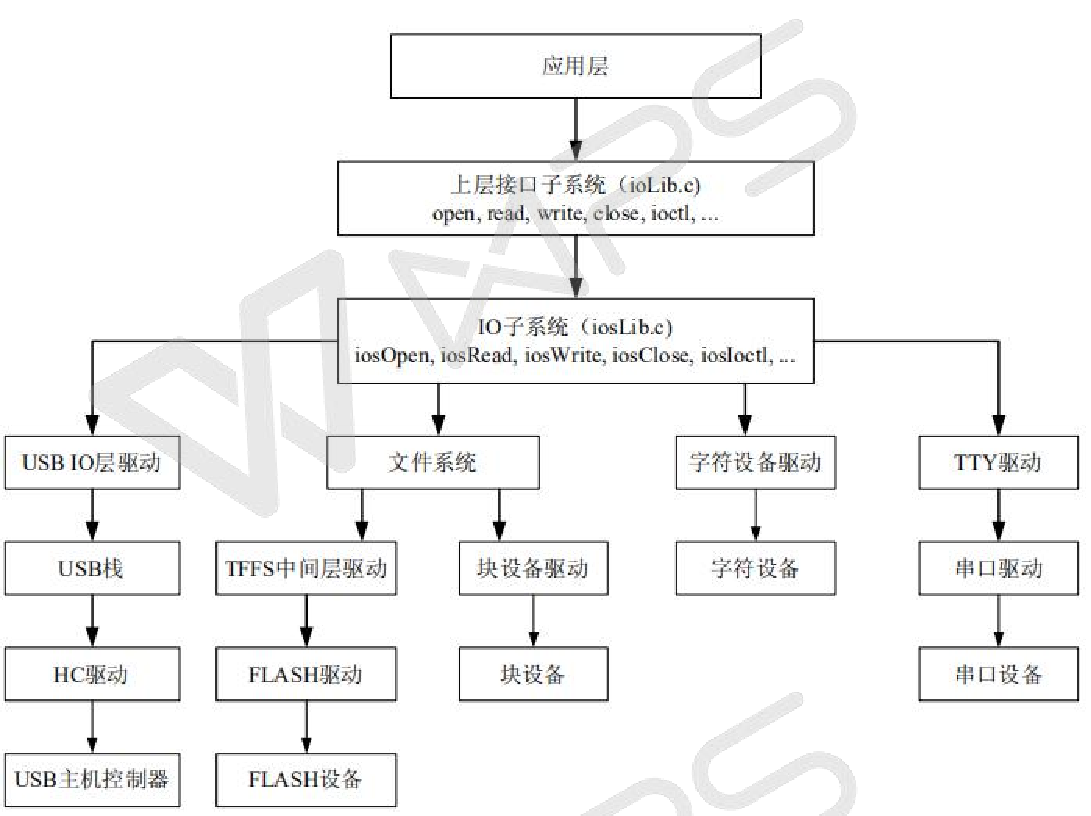
\includegraphics[width=1.0\textwidth]{./graphics/vxworks-kernel-diagram.pdf}
\caption{VxWorks驱动内核层次结构}\label{fig:VxWorks内核驱动层次结构}
\end{figure}
	
	I/O 子系统在整个驱动层次中起着十分重要的作用,其对下管理着各种类型的设备驱动。换句话说,各种类型(包括网络设备)的设备都必须向I/O 子系统进行注册方可被内核访问。所以在I/O 子系统这一层次,内核维护着三个十分关键的数组用以对设备所属驱动、设备本身以及当前系统文件句柄进行管理。需要指出的是,VxWorks文件系统在内核驱动层次中实际上是作为块设备驱动层次中的一个中间层而存在的,其向I/O 子系统进行注册,而将底层块设备驱动置于自身的管理之下以提高数据访问的效率。在这些文件系统中,dosFs 和rawFs 是最常用的两种文件系统类型,在VxWorks早期版本就包含对这两种文件系统的支持。
	
\section{内核驱动的相关结构}
\subsection{系统设备表}
	
	在VxWorks中对于每一个设备都会使用DEV\_ HDR的结构来表示这个设备,DEV\_ HDR的定义如下:
\lstset{language=C}
\begin{lstlisting}
/*h/iosLib.h*/
typedef struct /*DEV_HDR - device header for all device structures*/ 
{ 
  DL_NODE node; /* device linked list node */ 
  short drvNum; /* driver number for this device */ 
  char * name;/* device name */ 
}DEV_HDR;  
\end{lstlisting}

	在该结构中给出了链接指针node(用以将该结构串入队列中),驱动索引号drvNum,设备节点名name。内核提供这个结构较为简单,只存储了一些设备关键部分。底层驱动对其驱动的设备都有一个自定义数据结构表示,其中包含了被驱动设备寄存器基地址,中断号,可能的数据缓冲区,保存内核回调函数的指针,以及一些标志位。最为关键的一点是 DEV\_ HDR 内核结构必须是这个自定义数据结构的第一个成员变量,因为这个用户自定义结构最后需要添加到系统设备队列中,故必须能够在用户自定义结构与 DEV\_ HDR 结构之间进行转换,而将 DEV\_ HDR 结构设置为用户自定义结构的第一个成员变量就可以达到这个目的。
	
	
	驱动程序必须先将设备注册到 IO 子系统中,这个过程也被称为创建设备节点。IO子系统提供了一个简单的被驱动程序调用的设备注册函数iosDevAdd(),该函数原型如下:
\lstset{language=C}
\begin{lstlisting}
STATUS iosDevAdd 
( 
  DEV_HDR *pDevHdr, /* pointer to device's structure */ 
  char *name, /* name of device */ 
  int drvnum /* no. of servicing driver,returned by iosDrvInstall()*/
 ); 
\end{lstlisting}\\
iosDevAdd 函数将一个设备添加到由 IO 子系统维护的系统设备列表中,该列表是一个双向链表,成员通过指针链接在一起,这是由 DEV\_ HDR 结构中 node 成员变量完成的,每当添加设备时,系统都会像链表添加新的节点。系统设备列表由 iosDvList 内核变量指向,系统设备表在系统中的连接方式如\autoref{fig:VxWorks系统设备示意图}所示。系统设备表为open()、close()、remove()这三个函数提供文件与设备的连接,当应用程序执行这三个函数中的一个时,IO系统会将文件名和设备链表中的进行匹配,匹配成功之后就使用这个设备驱动进行文件的其他操作。

\begin{figure}[!h]
\centering
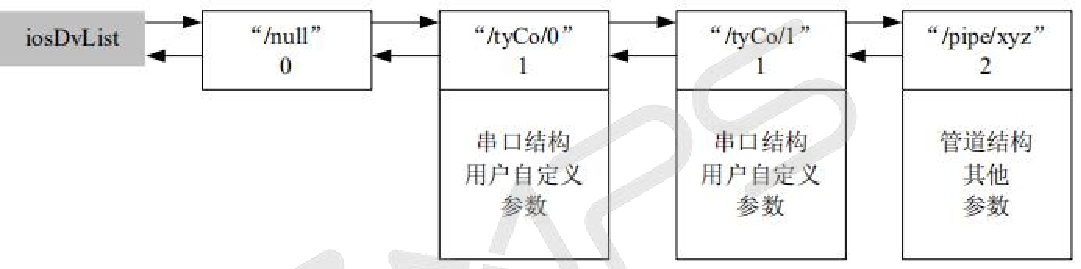
\includegraphics[width=1.0\textwidth]{./graphics/vxworks-device-link.pdf}
\caption{VxWorks系统设备示意图}\label{fig:VxWorks系统设备示意图}
\end{figure}

用户可以在命令行下使用iosDevShow或者是devs来显示系统设备的所有设备,在我们本次所使用的环境中,存在的设备如\autoref{fig:iosDevShow}所示。
\begin{figure}[!h]
\centering
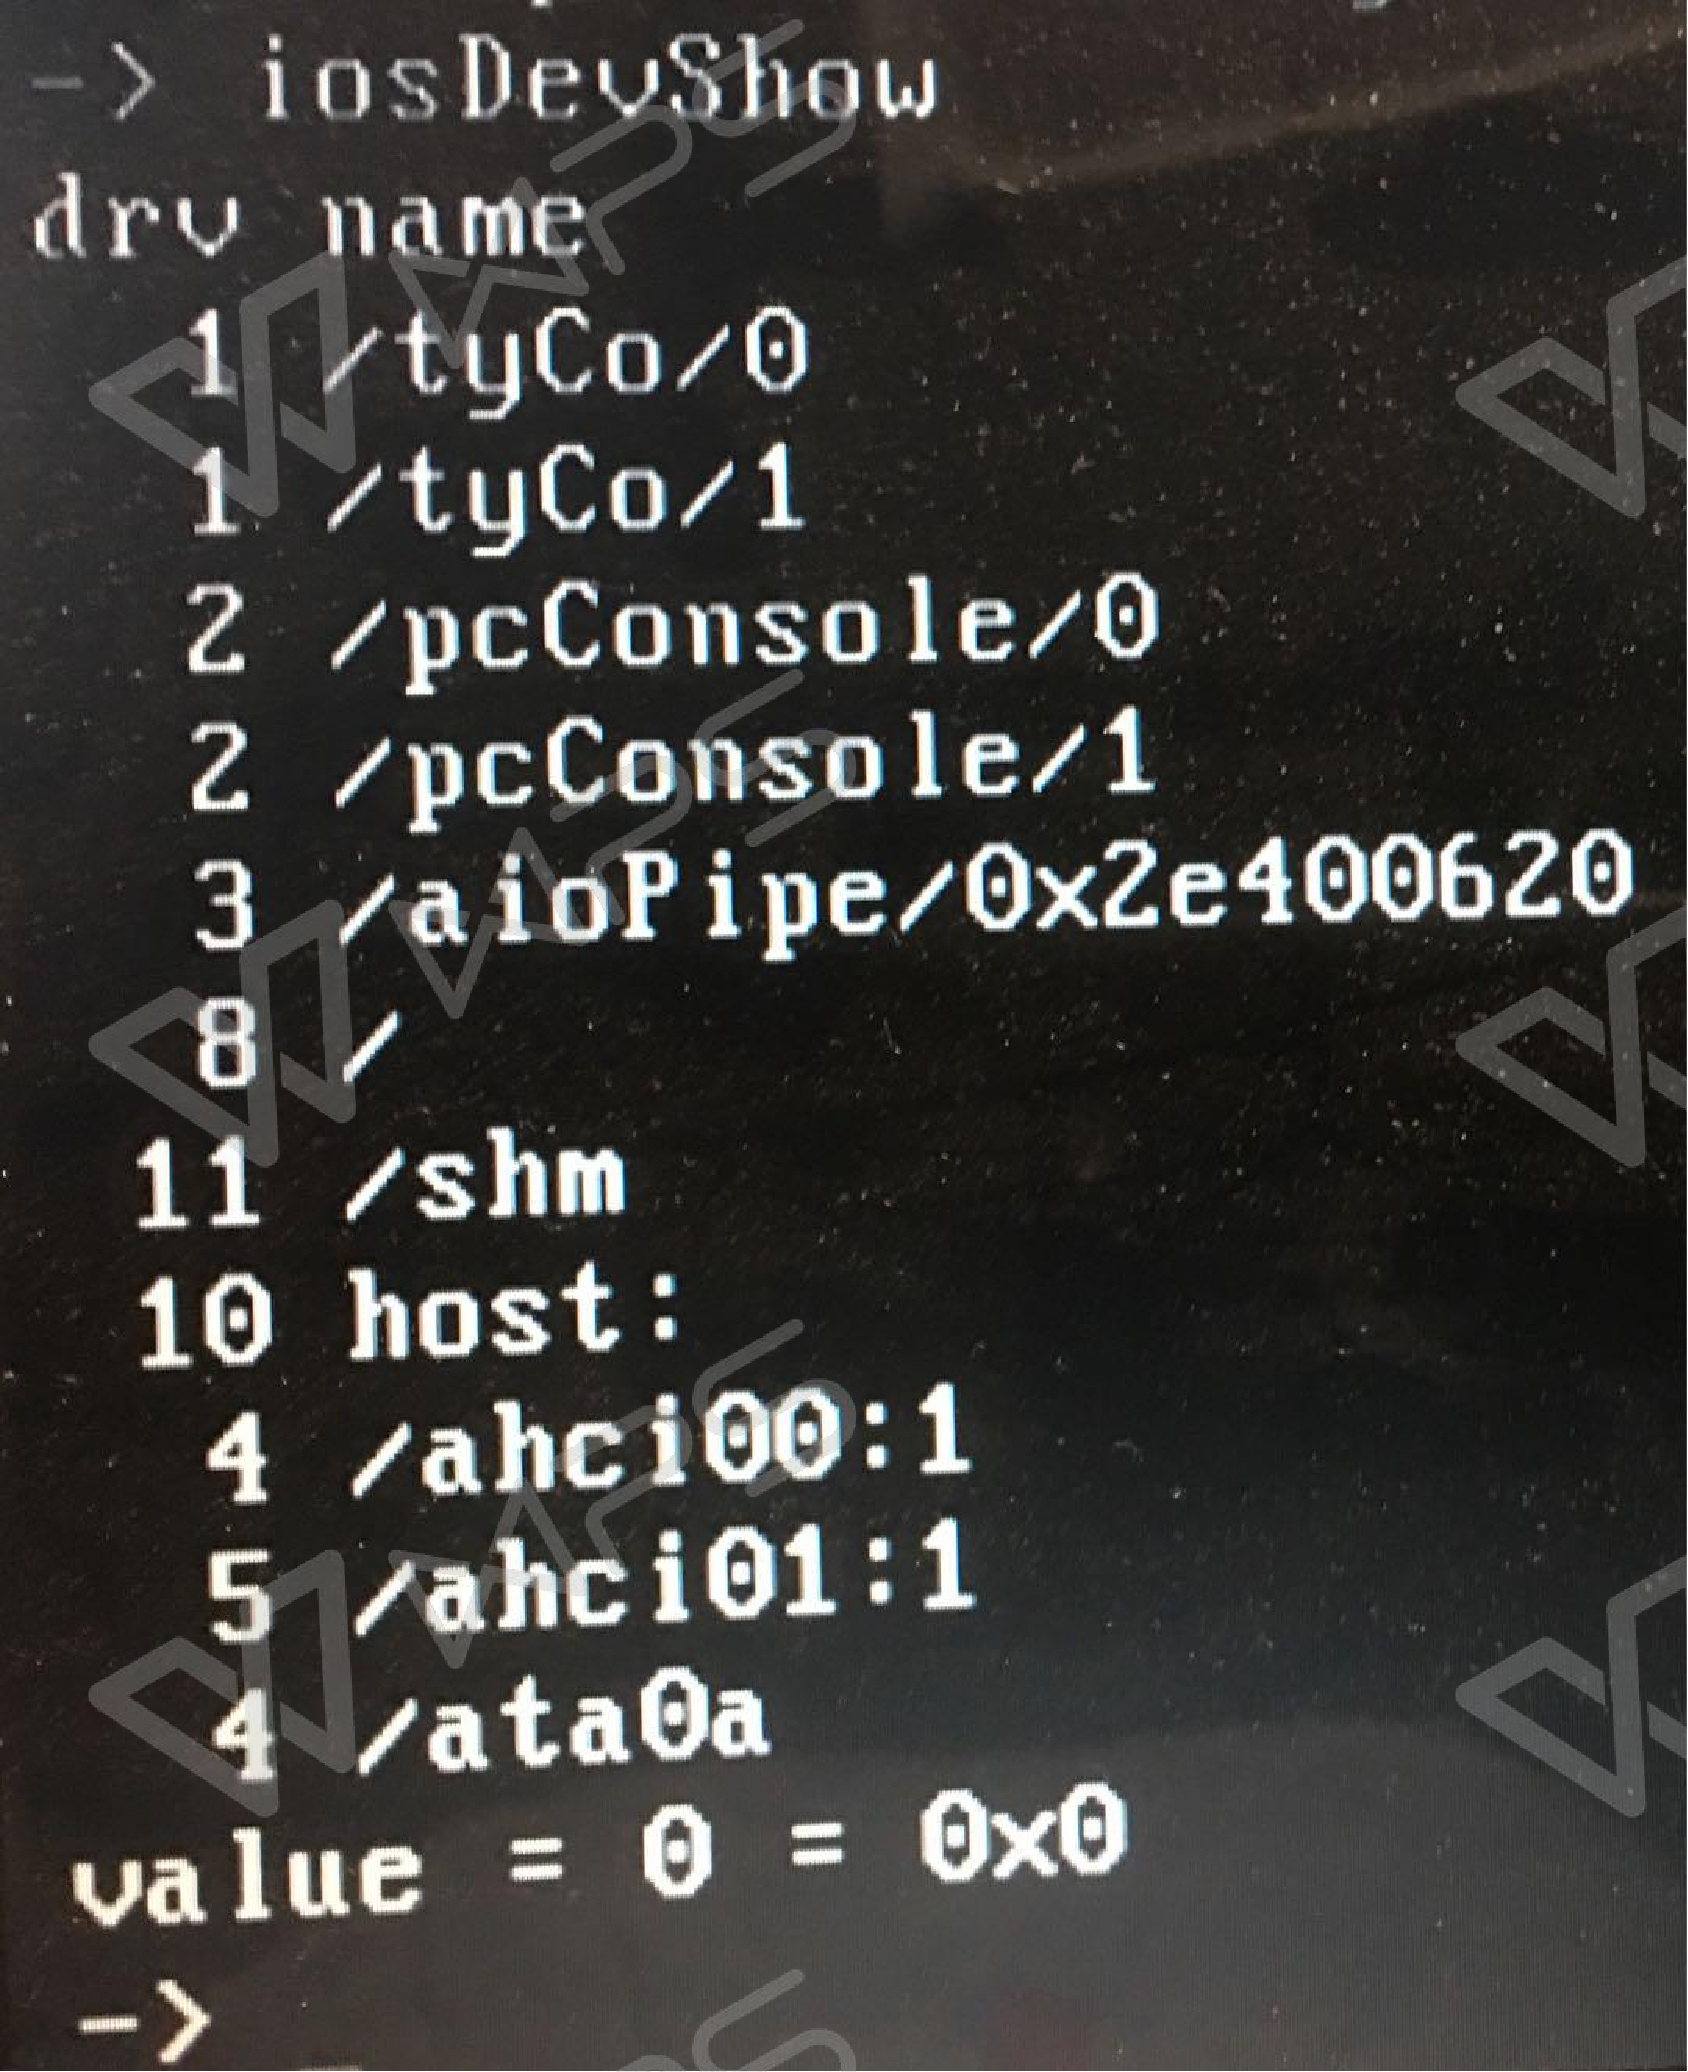
\includegraphics[width=.5\textwidth]{./graphics/iosDevShow.pdf}
\caption{当前系统上的所有设备}\label{fig:iosDevShow}
\end{figure}

\subsection{系统驱动表}

	\indent IO子系统维护的系统驱动表包含有当前注册到IO子系统下的所有驱动。这些驱动可以是直接驱动硬件工作的驱动层,如一般的字符驱动,也可以是驱动中间层,如文件系统中间层,TTY 中间层,USB IO 中间层等。对于中间层驱动,下层硬件驱动将由这些中间层自身负责管理,而不再通过 IO 子系统。如串口底层驱动将通过 TTY 中间层进行管理,而不再通过IO 子系统。
	
    \indent	系统驱动表底层的实现是一个数组,数组元素数目在 Vxworks 内核初始化过程中初始化 IO 子系统时指定,iosInit()函数用以初始化 IO 子系统,我们在编写驱动程序的时候不需要再调用此函数,因为内核已经帮我们初始化好了 IO 子系统。iosInit 函数调用原型如下:
\lstset{language=C}
\begin{lstlisting}
STATUS iosInit 
( 
  int max_drivers, /* maximum number of drivers allowed */ 
  int max_files, /* max number of files allowed open at once */ 
  char *nullDevName/* name of the null device (bit bucket) */ 
); 
\end{lstlisting}

在系统的驱动表中每一个表项都是一个 DRV\_ ENTRY 类型的结构,该结构定义在 h/private/iosLibP.h文件当中,其定义如下:
\lstset{language=C}
\begin{lstlisting}
typedef struct /* DRV_ENTRY - entries in driver jump table */ 
{ 
  FUNCPTR de_create; 
  FUNCPTR de_delete; 
  FUNCPTR de_open; 
  FUNCPTR de_close; 
  FUNCPTR de_read; 
  FUNCPTR de_write; 
  FUNCPTR de_ioctl; 
  BOOL de_inuse; 
} DRV_ENTRY; 
\end{lstlisting}
DEV\_ ENTRY结构体实际上就是一个函数指针结构,结构中每个成员都指向一个完成特定功能的函数,这些函数与用户层提供标准函数接口一一对应。成员 de\_ inuse 用以表示一个表项是否空闲。这个结构体中的函数指针实际指向的内容由驱动调用iosDrvInstall()来提供。 iosDrvInstall()是IO子系统提供的驱动程序注册函数,其原型如下:
\lstset{language=C}
\begin{lstlisting}
int iosDrvInstall 
( 
  FUNCPTR pCreate, /* pointer to driver create function */ 
  FUNCPTR pDelete, /* pointer to driver delete function */ 
  FUNCPTR pOpen, /* pointer to driver open function */ 
  FUNCPTR pClose, /* pointer to driver close function */ 
  FUNCPTR pRead, /* pointer to driver read function */ 
  FUNCPTR pWrite, /* pointer to driver write function */ 
  FUNCPTR pIoctl /* pointer to driver ioctl function */ 
); 
\end{lstlisting}
一个设备驱动在初始化过程中一方面完成硬件设备寄存器的配置,另一方面就是向 IO 子系统注册驱动和设备,从而使得设备对用户可见。可以看到 iosDrvInstall 函数参数为一系列函数地址,这些函数对应了为用户层提供的标准接口函数。一个驱动无需提供以上所有函数的实现,对于无需实现的函数,直接传递 NULL 指针即可。iosDrvInstall 函数基本实现即遍历drvTable 数组,查询一个空闲表项,用传入的函数地址对表项中各成员变量进行初始化,并将 de\_ inuse 设置为 TRUE,最后返回该表项在数组中的索引作为驱动号。设备初始化函数将使用该驱动号调用 iosDevAdd 将设备添加到 IO 子系统中。此后用户就可以使用 iosDevAdd函数调用时设置的设备节点名对设备进行打开操作,打开后进行读写或控制等其他操作,完成用户要求的特定功能。

	用户可在命令行下输入 iosDrvShow,显示系统驱动表中当前存储的所有驱动。如\autoref{fig:iosDrvShow}所示为当前系统中的所有驱动。
\begin{figure}[!h]
\centering
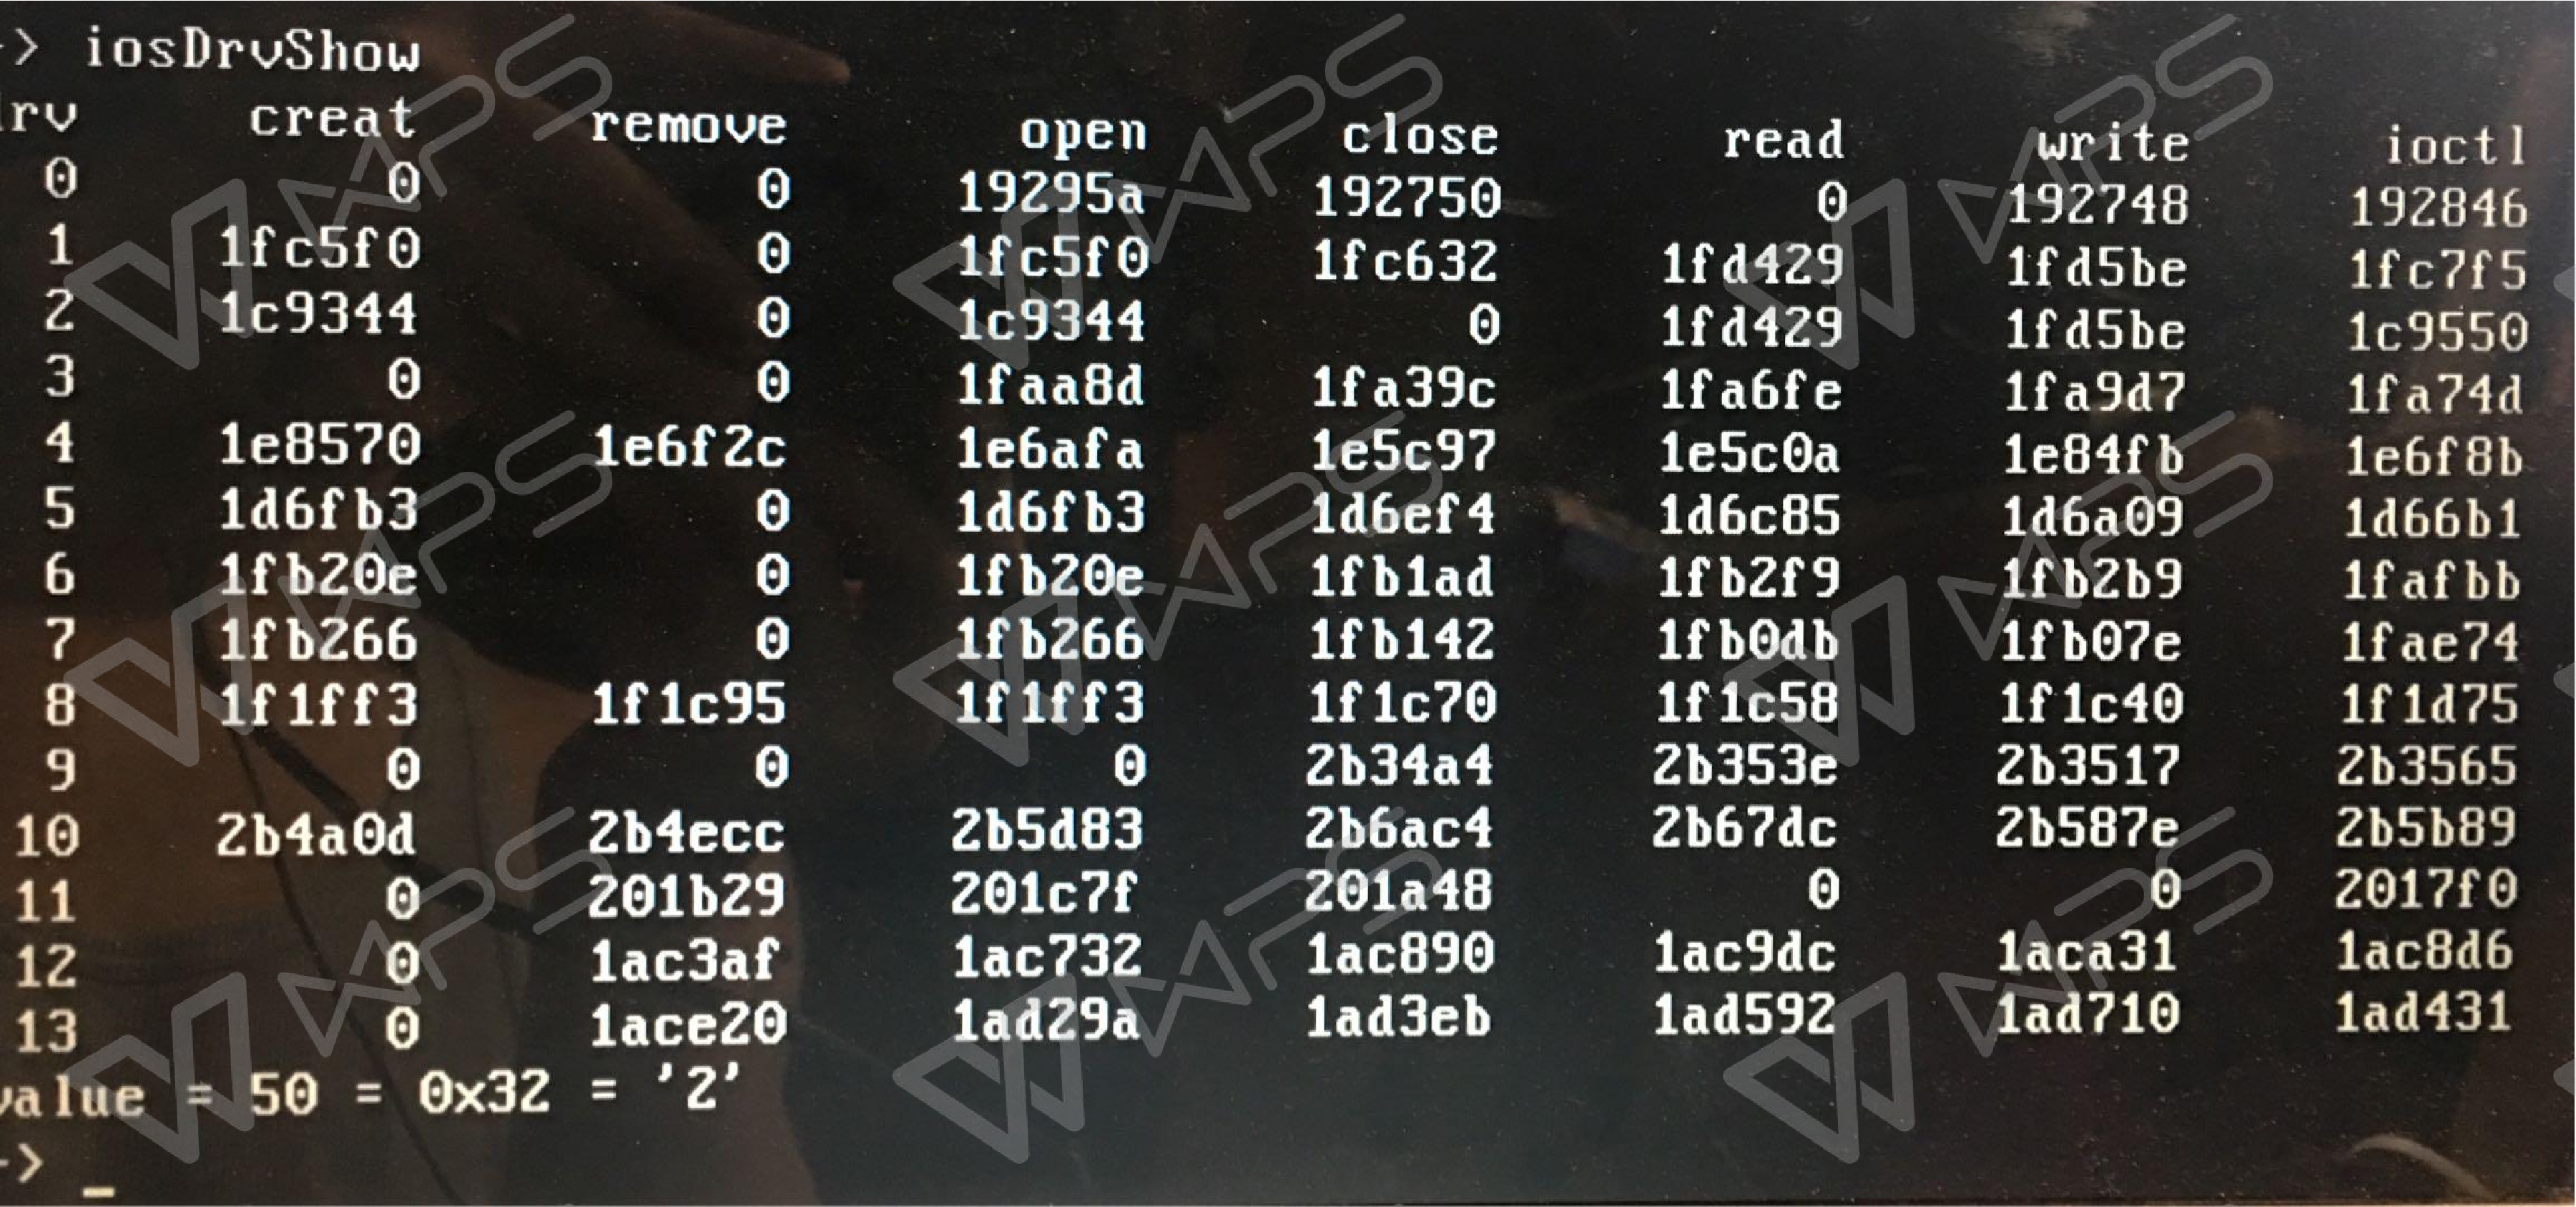
\includegraphics[width=.9\textwidth]{./graphics/iosDrvShow.pdf}
\caption{当前系统上的驱动表}\label{fig:iosDrvShow}
\end{figure}

\subsection{系统文件描述符表}
	系统描述符表存储着当前系统范围内打开的所有文件的描述符。文件描述符表底层实现上也是一个数组,正如设备驱动表表项索引用作驱动号,文件描述符表表项索引被用作文件描述符 ID,即 open 函数返回值。对于文件描述符有一点需要注意:标准输入,标准输出,标准错误输出虽然使用 0,1,2 三个文件描述符,但是可能在系统文件描述附表中只占用一个表项,即都使用同一个表项。Vxworks 内核将 0,1,2 三个标准文件描述符与系统文件描述符表中内容分开进行管理。实际上系统文件描述符中的内容更多的是针对硬件设备,即使用一次 open 函数调用就占用一个表项。0,1,2 三个标准文件描述符虽然占用 ID 空间(即其他描述符此时只能从 3 开始分配),但是其只使用了一次 open 函数调用,此后使用 ioGlobalStdSet 函数对 open 返回值进行了复制。
	
	系统文件描述符表中每个表项都是一个 FD\_ ENTRY 类型的结构,该结构定义在h/private/iosLibP.h 中,如下所示。
\lstset{language=C}
\begin{lstlisting}
typedef struct /* FD_ENTRY - entries in file table */ 
{ 
  DEV_HDR * pDevHdr;/* device header for this file */ 
  int value; /* driver's id for this file */ 
  char * name; /* actual file name */ 
  int taskId; /* task to receive SIGIO when enabled */ 
  BOOL inuse; /* active entry */ 
  BOOL obsolete; /* underlying driver has been deleted */ 
  void * auxValue;/* driver specific ptr, e.g. socket type */ 
  void * reserved; /* reserved for driver use */ 
} FD_ENTRY; 
\end{lstlisting}

用户程序每调用一次 open 函数,系统文件描述符表中就增加一个有效表项,直到数组满,此时 open函数调用将以失败返回。表项在表中的索引偏移 3 后作为文件描述符返回给用户,作为接下来其他所有操作的文件句柄。用户可以通过iosFdShow来显示系统文件描述符表中当前所有的有效表项,如\autoref{fig:iosFdShow}所示是当前系统下的文件系统描述符表。
\begin{figure}[!h]
\centering
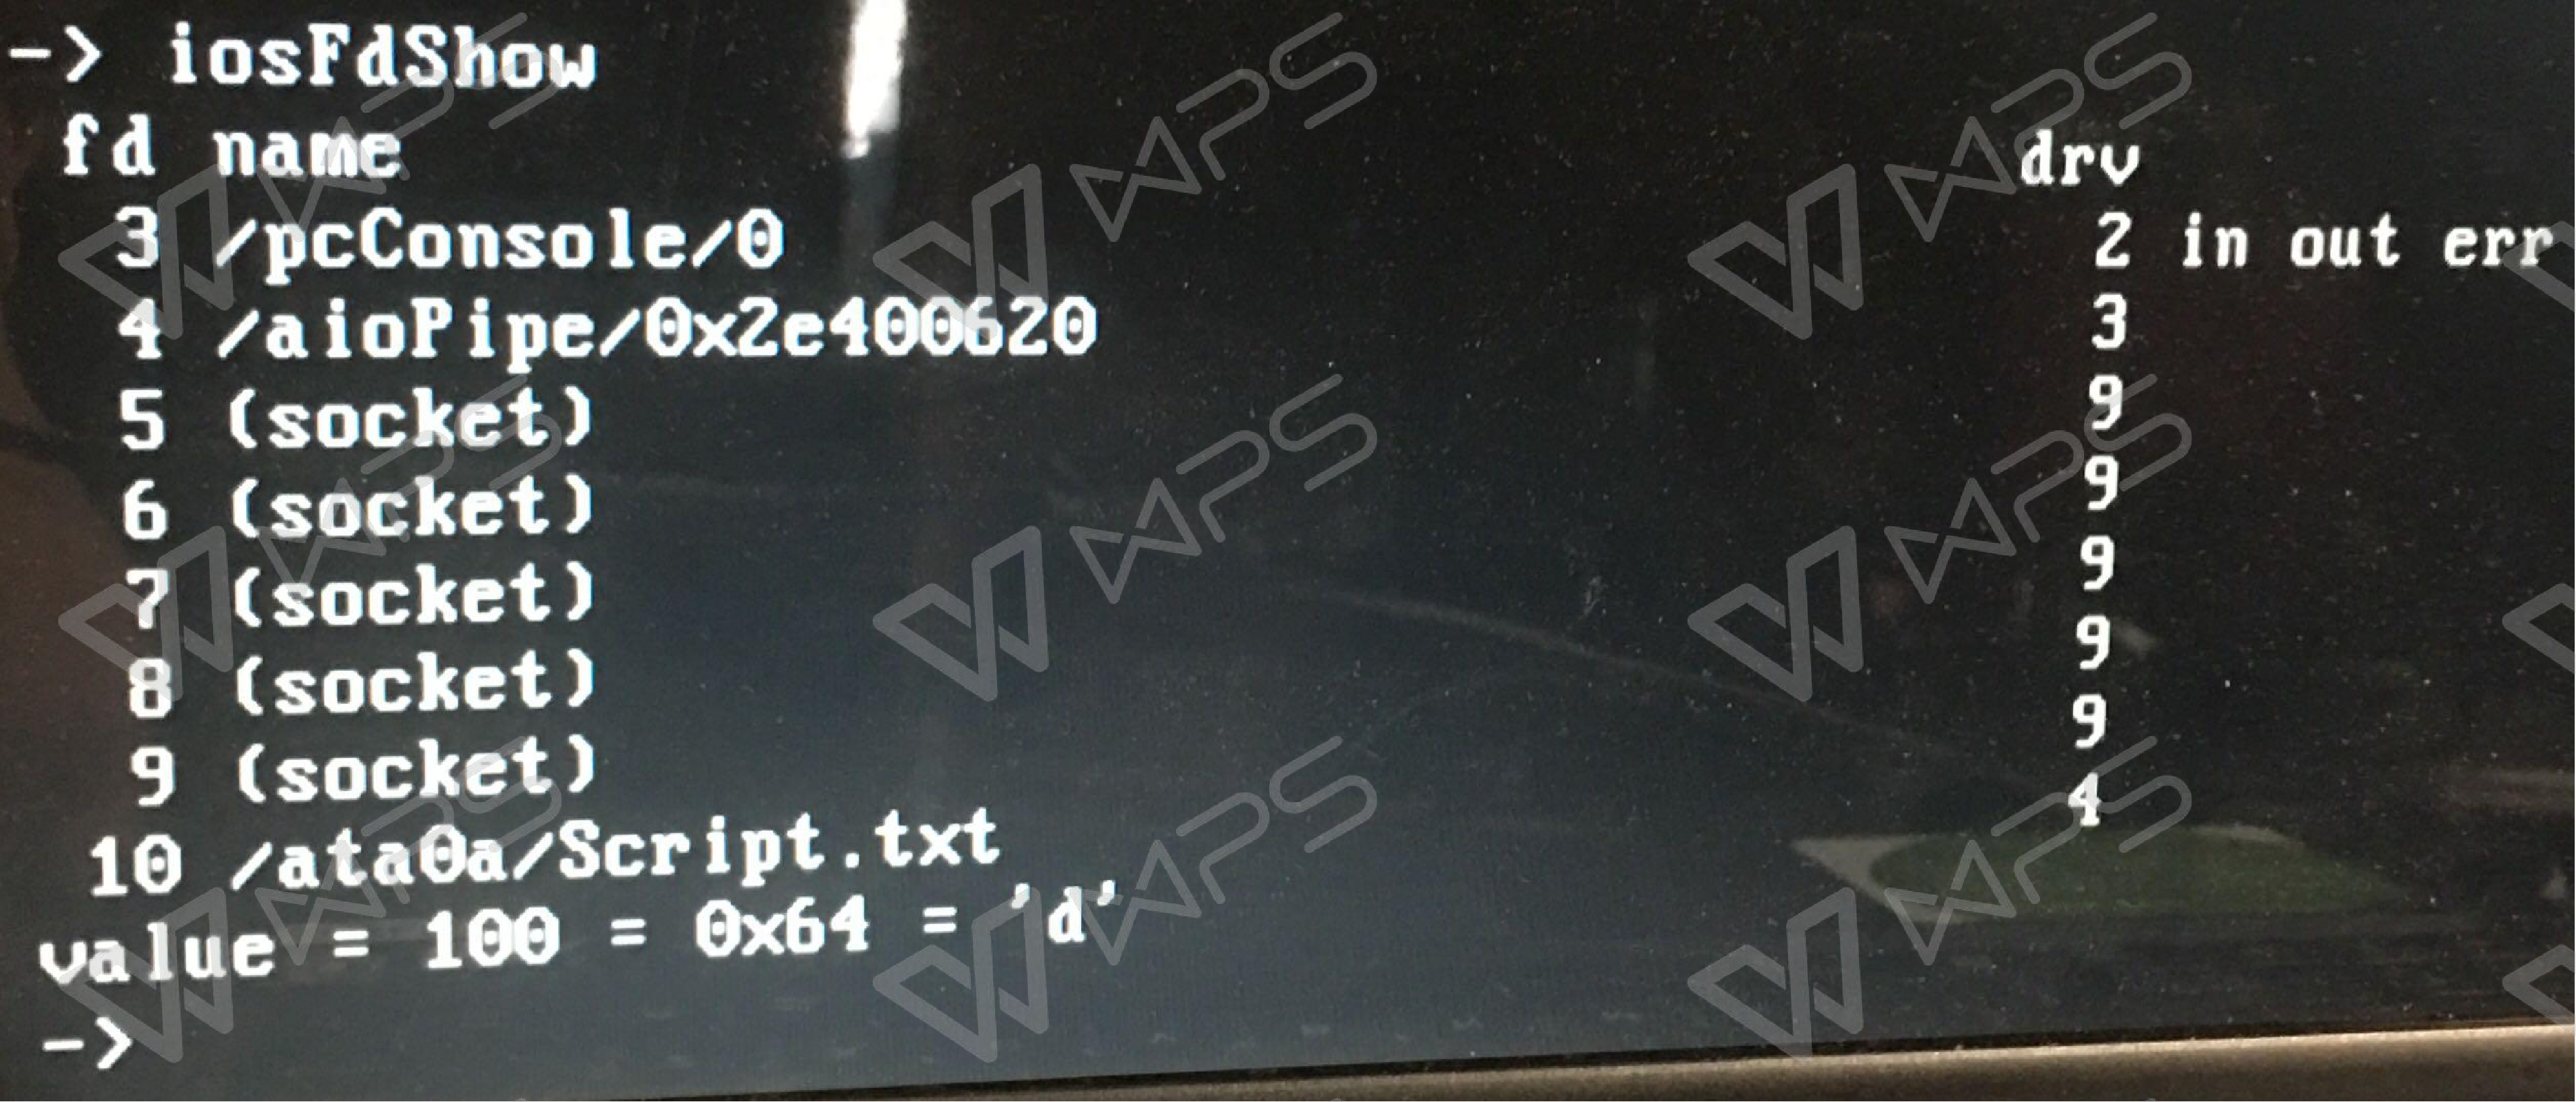
\includegraphics[width=.9\textwidth]{./graphics/iosFdShow.pdf}
\caption{当前系统上的文件描述符表}\label{fig:iosFdShow}
\end{figure}

\section{USB转串口设备驱动程序的实现}
	VxWorks调试通道当中运行的最主要的软件平台是嵌入式实时操作系统VxWorks,作为系统的最底层的软件,要想进行数据的传输,驱动程序是必不可少的。本系统中的硬件设备是基于USB总线的,USB口转串口设备的驱动程序在Windows和Linux下都有现成可用的,但是在VxWorks下需要自己来实现这部分。
	
\subsection{VxWorks上的USB协议栈}
	VxWorks的USB主机驱动程序堆栈满足USB协议规定的要求,提供了一整套服务来操作USB以及一些预置USB类驱动程序,以处理特定类型的USB设备。在Wind River的VxWorks中USB驱动程序堆栈的开发符合的是通用串行总线规范2.0版,USB系统是一种主从结构,系统的所有动作都是由USB主机发起,并协调不同的设备动作,设备端软件在系统中只需要对主机的命令做出响应即可,USB的主机端由于在系统中的地位比较特殊,因而其软件结构比较复杂,USB协议在主机端是分层实现的,其通信的逻辑结构和PC端的软硬件结构如\autoref{fig:usb通信结构}所示。USB协议由上至下可以分为三层:客户端驱动程序(Client Driver)、USB驱动(USBD)、主机控制器驱动(HCD),每一层完成不同的功能。

\begin{figure}[h]
\centering
  \begin{subfigure}[b]{0.4\textwidth}
  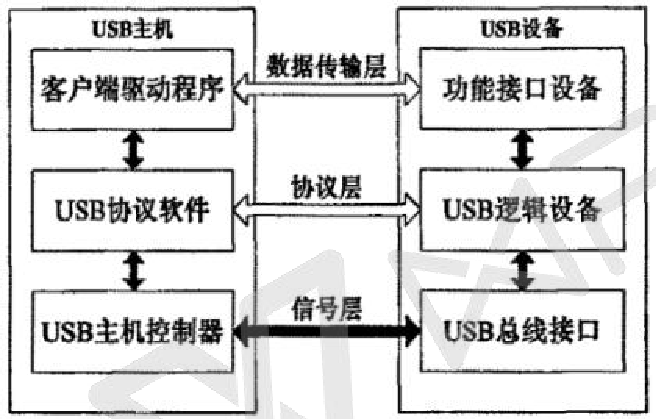
\includegraphics[width=1.0\textwidth]{./graphics/USB-device-structure-diagram.pdf}
  \caption{USB通信的逻辑结构}\label{fig:usb通信逻辑结构}
  \end{subfigure}
  ~
  \begin{subfigure}[b]{0.5\textwidth}
  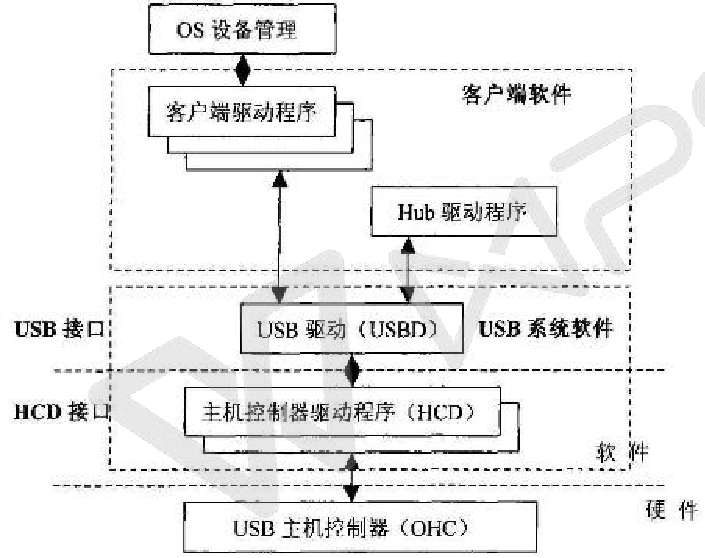
\includegraphics[width=1.0\textwidth]{./graphics/USB-PC-structure.pdf}
  \caption{USB主机端软硬件结构}\label{fig:usb-PC}
  \end{subfigure}
\caption{USB通信结构}\label{fig:USB通信结构}
\end{figure}
	
	客户端驱动程序完成对不同的设备类的设备的功能驱动。本次设计中所要完成的USB口转串口的驱动要完成的就是客户端驱动。为了和设备进行正常的通信,他通过USB的I/O请求包(I/O request,IRP)向USBD层发出数据接收或者发送的请求。此外,USB的传输机制对于客户端的驱动程序而言是完全透明的,客户端驱动程序所看到的仅仅是具体的设备类,不管设备采用的何种的数据传输方式。另外IRP是USB协议定义的抽象概念,其结构需要根据协议的具体来实现。
	
	USBD是USB的核心驱动,其提供的功能包括USB总线的枚举、总线带宽的分配、传输控制等操作。向上的接口负责处理客户端驱动程序提出的I/O请求,他通过IRP了解此设备的属性和本次数据通信的具体要求,将此IRP转换成USB能够识别的一系列的事物处理,交给HCD层或直接交给主机控制器处理。USBD还负责新设备的动态插拔、USB电源管理和对客户端驱动程序的维护等操作。
	
	HCD层的主要功能是与主机控制器合作完成USB的各种事物处理。它根据一定的规则调度所有奖杯广播发送到USB上的事物处理。调度方法是首先将数据传输类型组成不同的链表,每一种链表包括来自不同的设备驱动程序的同一种类型的数据,然后定义不同的数据类型在传输中所占的带宽比例,交给主机控制器处理,控制器根据规则从立案表上摘下数据块,根据大小为它创建一个或者多个事物处理,完成与设备的数据传输,当事物处理完成时HCD将结果交给USBD层。此外它还完成对主机控制器和根集线器的配置和驱动等操作。WindRiver提供了两种类型的主机控制器驱动:usbHcdUhciLib(UHCI主机控制器驱动)和usbHcdOhciLib(OHCI主机控制器驱动)。VxWorks的USBD和HCD之间的接口允许操过一个的底层主控制器,并且USBD能够同时连接多个USB HCD。这样的设计特点可以让开发者建立复杂的USB系统。

	在VxWorks系统当中UBSD层的驱动和HCD层的驱动都是已经实现好的,我们所需要实现的是客户端的驱动程序,用以驱动特定的USB设备。	


\subsection{特定需求单设备驱动的实现}

	由于对于仅支持单设备驱动程序是基于特定的需求而具体定制的,所以该设备的驱动程序的实现流程与通常的支持多设备的驱动的初始化流程存在差异。具体的需求为:
\hei{驱动中支持的设备名是固定的,驱动程序中要有缓存一定数据的能力,即使设备没有正确的连接也要能够往这个驱动中写入数据,并且一旦设备连接之后就能够将驱动中缓存的数据发送出去。}

	由于需要在设备未连接时就能够往设备中写入数据,且设备名为固定的,那么就必须调整驱动的初始化流程,使得其能够支持这一特性,通常驱动都是在设备加载之后再将其加入到系统设备表和系统驱动表当中,那么此时我们就需要先将一个固定的设备名加入到系统设备表当中。对于该特定需求的单设备驱动的流程图如\autoref{fig:single-usb-rs232drv-structure}所示。
\begin{figure}[!ht]
\centering
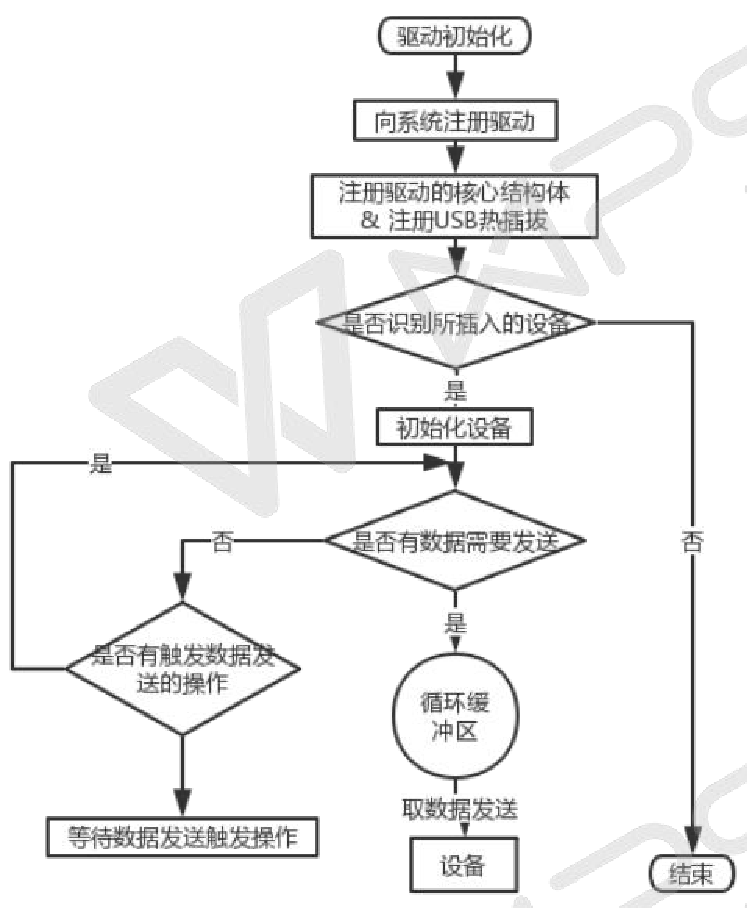
\includegraphics[width=.7\textwidth]{./graphics/sDevDrv.pdf}
\caption{特定需求的驱动流程图}\label{fig:single-usb-rs232drv-structure}
\end{figure}


\subsubsection{驱动的设备结构}
	底层驱动都要对其驱动的设备维护一个结构,用以保存设备的关键参数:USB配置、接口、端点地址、读写缓冲区的指针等等,这些信息将随着设备类型的不同而有所差别。对于我们此处要驱动的USB口转串口驱动,我们驱动中的关键数据结构如下: 
	
\lstset{language=C}
\begin{lstlisting}
typedef struct cp210x_dev
{
  DEV_HDR cp210xDevHdr; /*must be first field*/
  LINK 	devHdrLink;/*linked list of  devhdr structs*/
  UINT16                  numOpen;
  USBD_NODE_ID nodeId;			/*device nodeID*/
  UINT16 configuration;	/*configuration/interface reported as*/
  UINT16 interface;		/*a interface of this device*/
  UINT16 interfaceAltSetting;
  UINT16 vendorId;
  UINT16 productId;

  BOOL connected;
  USBD_PIPE_HANDLE outPipeHandle; /* USBD pipe handle for bulk OUT pipe */
  USB_IRP	outIrp;					/*IRP to monitor output to device*/
  BOOL outIrpInUse;
  UINT32 outErrors;				/*TRUE while IRP is outstanding*/
  UINT16  outEpAddr;	
  int trans_len;
  UINT8 trans_buf[64];
  
  USBD_PIPE_HANDLE inPipeHandle;
  USB_IRP inIrp;
  BOOL inIrpInUse;
  UINT8 inBuf[64];
  UINT32 inErrors;
  UINT16 	inEpAddr;
	
  char *writeBuf;
  int writeFront;
  int writeRear;
  char *readBuf;
  int readFront;
  int readRear;
} CP210X_DEV, *pCP210XDEV;
\end{lstlisting}
\noindent 部分成员的含义如下:

\begin{itemize}
\item DEV\_ HDR:自定义设备结构的第一个成员必须是DEV\_ HDR结构类型,对于内核的I/O子系统而言,其将所有的设备结构都看作是DEV\_ HDR类型,内核仅仅对DEV\_ HDR结构进行管理,在系统的设备列表中,内核只使用DEV\_ HDR结构当中的成员。自定义结构中的其他成员由驱动自己使用,内核并不了解这些自定义成员。
\item numOpen:用来记录设备被打开的次数,每次调用open()函数打开该设备则numOpen加一,调用close()函数关闭设备则减一。
\item nodeId:用来保存该设备在系统中的唯一ID号。
\item configure、interface、interfaceAltsetting:用来保存设备的描述符中的配置、接口、可变接口信息。
\item vendorId、productId:保存该设备的厂商ID和产品ID,用来识别该设备是否适合我们的驱动程序。
\item outPipeHandle、inPipeHandle:设备的输入/输出端点的管道句柄,每次传输数据时都需要使用该句柄来表明数据传到的哪一个端点。
\end{itemize}

\subsubsection{驱动注册和设备创建} 
	
	底层驱动一般提供形如 xxxDrv 和 xxxDevCreate 之类的函数完成驱动注册和设备创建的工作。这些工作的完成一般是在内核启动过程中进行。对于此处的USB口转串口驱动我们定义cp210xDrvInit() 初始化函数,其主要完成驱动所需要的资源申请和系统的初始化,包括创建信号量、向系统注册驱动、创建设备、向USBD层注册。cp210xDevInit模块主要代码如下所示:
\lstset{language=C}
\begin{lstlisting}
STATUS cp210xDrvInit(void)
{
  ...
  if(OSS_MUTEX_CREATE(&cp210xWriteMutex) != OK || OSS_MUTEX_CREATE(&cp210xReadMutex) != OK || OSS_MUTEX_CREATE(&cp210xMutex) != OK || (blockReadSem = semBCreate(SEM_Q_FIFO, SEM_EMPTY)) == NULL )
  ... 	
  cp210xDrvNum = iosDrvInstall(NULL,NULL,cp210xDevOpen,cp210xDevClose,
			cp210xDevRead,cp210xDevWrite,cp210xDevIoctl);
  ...
  if( iosDevAdd(&pCp210xDev->cp210xDevHdr,CP210X_NAME,cp210xDrvNum) != OK)
  ...  
  if(usbdClientRegister (CP210X_CLIENT_NAME, &cp210xHandle) != OK)
  ...  
  if(usbdDynamicAttachRegister(cp210xHandle,USBD_NOTIFY_ALL,USBD_NOTIFY_ALL,USBD_NOTIFY_ALL,TRUE,(USBD_ATTACH_CALLBACK)cp210xAttachCallback)!= OK)
  ...
}
\end{lstlisting}\\

	驱动会在进入初始化的时候首先检查该驱动是否已经安装,若已经安装了则无需再次安装,直接退出即可,cp210xDrvInit()通常是在usrRoot(usrConfig.c)中调用,但是你也可以手动调用这个函数对该驱动进行初始化操作。然后会进行一些驱动所需要的全局资源的初始化,如信号量、全局变量、看门狗等,接着调用iosDrvInstall()函数安装驱动的I/O函数,将其添加到驱动表当中,在我们的USB口转串口驱动当中不需要实现delete函数和create函数,直接将其指针置为NULL即可。
	
	注册完成之后还要向系统将该驱动程序添加到IO子系统当中,添加成功后会在系统的设备列表中显示该命名为CP210X\_ NAME的设备(CP210X\_ NAME只是一个宏定义,设备名可以自己更改)。此处即是我们的驱动程序中的一个特殊的地方,在没有识别到设备之前就已经创建好设备文件,只不过此时该设备还只是一个“假”的,只有软件实现,没有硬件支撑,即使此时已经可以打开该设备,向该设备写入数据,但是也只是写入到了系统的缓冲区当中而已,数据并没有发送到任何的硬件上。在驱动的内部我们会建立一个循环缓冲区来接收上层程序写入的数据,若系统中没有USB口转串口的设备,那么所有的数据就只会写入到该循环缓冲区当中,当循环缓冲区中的数据已经满了之后,遵循先进先出的原则来覆盖数据。当USB口转串口设备连接上时,若循环缓冲区当中已经有数据存在,则会立即启动发送数据的过程,若没有数据,则什么也不做。循环缓冲区的结构/功能如\autoref{fig:recruit-buffer-diagram}所示。
\begin{figure}[!h]
\centering
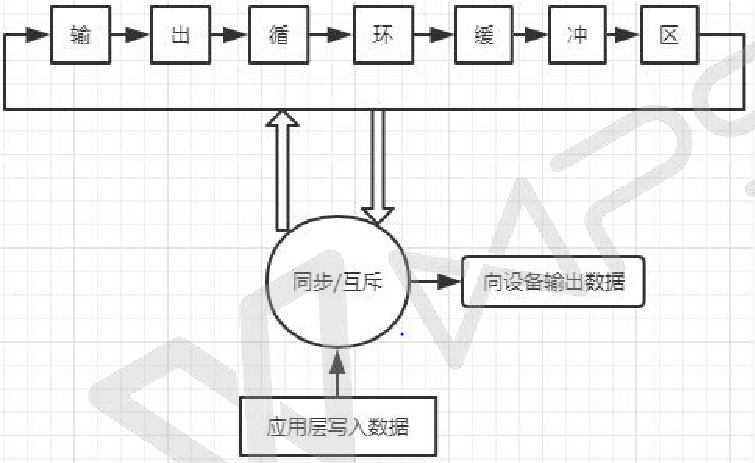
\includegraphics[width=.9\textwidth]{./graphics/recruit-buffer-diagram.pdf}
\caption{循环缓冲区结构/功能图}\label{fig:recruit-buffer-diagram}
\end{figure}

	接下来USB客户端驱动还需要向USBD层注册,注册完成之后会返回一个用于操作USBD的客户端handle,我们将其保存在cp210xHandle这个变量当中。然后还要注册一个动态注册的回调函数,当USBD层发现有USB设备的插拔动作时,就会根据我们注册时选定的设备类和接口类来判断是否需要调用我们注册的回调函数,由于我们的设备是一个特殊的设备,并不符合任何标准的USB设备类和接口类,于是我们将这两个参数置为USBD\_ NOTIFY\_ ALL,即任何USB设备的插拔都调用我们的注册的回调函数。之后我们在回调函数中根据设备的vendorId和productId来判断其是否是我们的驱动支持的设备,本驱动支持的设备的productId和vendorId存储在一个二维数组当中,判断过程是即遍历当前插入的设备的VID和PID是否在我们的数组当中。设备识别的流程如\autoref{fig:device-recognize}所示,目前支持的设备的设备ID、产品ID的组合如\autoref{tab:目前支持的设备列表}所示。

\begin{figure}[!h]
\centering
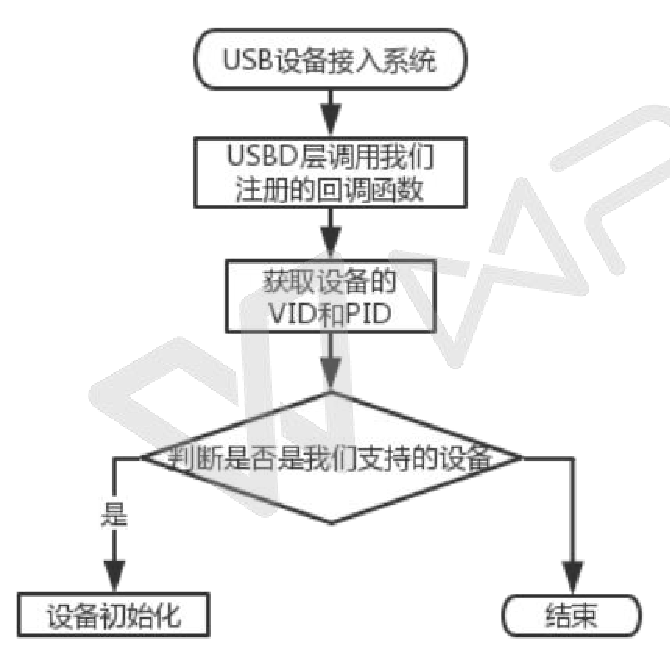
\includegraphics[width=.9\textwidth]{./graphics/device-recognize.pdf}
\caption{设备识别流程图}\label{fig:device-recognize}
\end{figure}


\begin{table}[!h]
\centering
\begin{tabular}{|c|c|c|c|c|c|c|}
\hline
{\hei{PID}}&{0x045B}&{0x0471}&{0x0489}&{0x0489}&{0x10C4}&{0x10C4}\\ 
\hline
{\hei{VID}}&{0x0053}&{0x066A}&{0xE000}&{0xE003}&{0x80F6}&{0x8115}\\
\hline 
{\hei{PID}}&{0x10C4}&{0x10C4}&{0x10C4}&{0x10C4}&{0x10C4}&{0x2405}\\
\hline
{\hei{VID}}&{0xEA60}&{0x813D}&{0x813F}&{0x814A}&{0x814B}&{0x0003}\\
\hline
\end{tabular}
\caption{目前支持的设备列表}\label{tab:目前支持的设备列表}
\end{table}

\subsubsection{设备的初始化}

设备的初始化包括获取该USB设备的各种描述符信息。包括设备描述符信息、配置描述符信息、接口描述符信息、端点描述符信息。再通过所获得的这些信息来创建到输出端点的管道和对设备进行设置,我们在此处将设备的波特率初始化为115200,数据位为8位,1个停止位,没有奇偶校验,没有流控。设备的初始化流程图如\autoref{fig:device-init}所示。

\begin{figure}[!h]
\centering
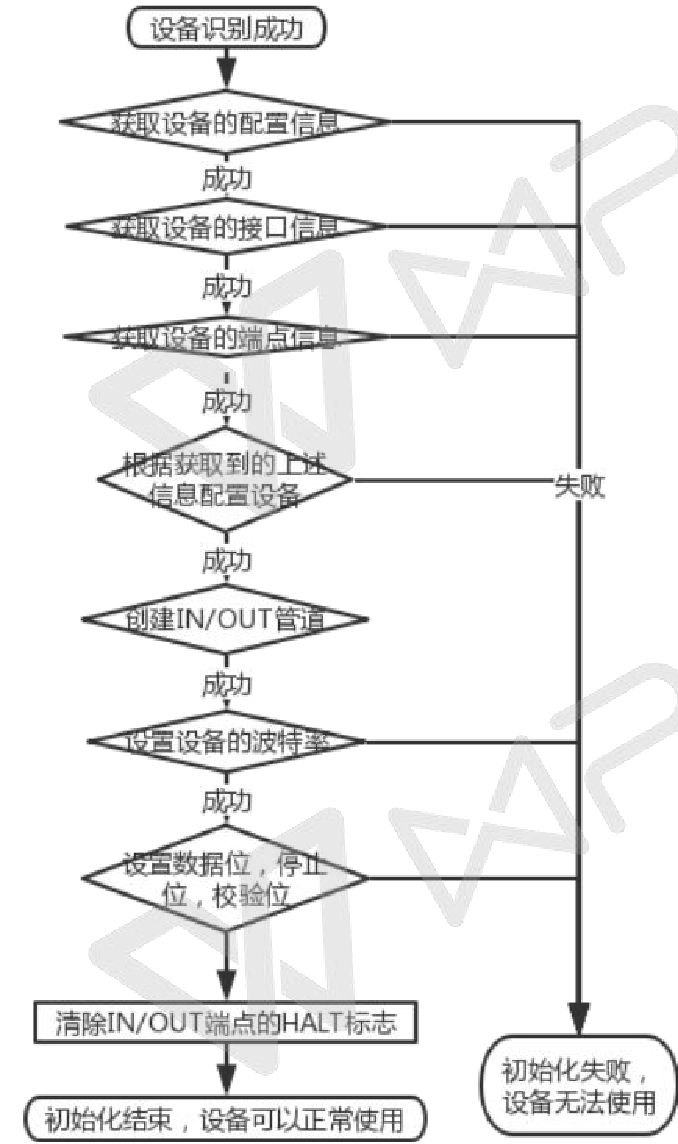
\includegraphics[width=.4\textwidth]{./graphics/device-init.pdf}
\caption{设备初始化流程图}\label{fig:device-init}
\end{figure}



\subsubsection{设备打开/关闭函数}

	用户在使用一个设备之前必须先打开这个设备,底层驱动响应函数中根据设备的需要将进行中断注册和使能设备工作配置等操作。对于我们的USB口转串口驱动而言,我们不需要自己管理中断,USBD层会为我们进行中断的管理工作,而配置工作我们在设备的初始化工作中已经完成,因此此处我们的设备打开工作,只需要简单的记录设备被打开的次数,并返回一个文件描述符即可。代码如下所示:
	
\lstset{language=C}
\begin{lstlisting}
LOCAL CP210X_DEV * cp210xDevOpen(DEV_HDR *pDevHdr, char *name, int flags,int mode)
{
	CP210X_DEV *pCp210xDev;
	pCp210xDev = (CP210X_DEV *)pDevHdr;
	(pCp210xDev->numOpen)++;
	return (pCp210xDev);
}
\end{lstlisting}


	需要注意的是第一个参数是由 IO 子系统提供的,IO 子系统在根据驱动号寻址到对应驱动函数时,其将系统设备列表中存储的设备结构作为第一个参数调用 cp210xDevOpen。实际上该参数是一个 CP210X\_ DEV 结构类型,但是 IO 子系统只认识DEV\_ HDR 结构。所以在 cp210xDevOpen函数中我们需要首先将这个 DEV\_ HDR 结构转换成 SPI\_ DEV,这基本上是所有底层驱动函数实现中第一条语句需要完成的任务。当然,驱动程序员也可以直接将第一个参数的类型设置为自定义结构类型,那么对于我们USB口转串口驱动,以上  cp210xDevOpen 函数的调用原型就变为:LOCAL int cp210xDevOpen(CP210X\_ DEV *pCp210xDev, char *name, int flags,int mode)这并不会造成什么影响,因为 IO 子系统传递过来实际上就是 CP210X\_ DEV 结构类型,只不过 IO 子系统对于驱动自定义参数并不关心,其只需要对 DEV\_ HDR 进行操作就可满足 IO 子系统本身管理的需要,其他自定义参数完全由底层驱动本身进行解释和使用。
	
	第二个参数是设备名匹配后的剩余部分,在我们的应用中,由于 open 函数调用时输入的路径名与系统设备列表中的设备名完全匹配,故此处的 name 应为空字符串。但是对于在文件系统层下的块设备而言,此处 name 指向的就是块设备节点名后的子目录和文件名。

	第三,四个参数就是用户 open 调用时传入的第二,三个参数,IO 子系统原封不动的将他们传递给了 cp210xDevOpen 函数。
	
	返回值为CP210X\_ DEV结构类型,一般返回如下两种值:一个有效的CP210X\_ DEV结构指针表示 cp210xDevOpen 调用成功,ERROR 则表示 cp210xDevOpen 调用失败,IO 子系统根据有效指针或者ERROR 返回一个文件描述符或者返回错误。cp210xDevOpen 函数的返回值非常重要,这个指针将被 IO 子系统保存,用于其后对驱动中读写,控制函数的调用。这个返回的指针将作为这些函数的第一个参数。
	
	设备的关闭和设备的打开操作是相反的操作,在关闭操作当中我们只需要对设备记录的打开次数进行减法操作即可。

\subsubsection{设备的读写}
	在成功打开一个设备后,用户程序将得到一个文件描述符,此后用户就可以使用这个文件描述符对设备进行读写,控制操作。底层驱动读写函数原型如下。

\lstset{language=C}
\begin{lstlisting}
LOCAL int cp210xDevWrite(CP210X_DEV *pCp210xDev, char *buffer,UINT32 nBytes)
LOCAL int cp210xDevRead(CP210X_DEV *pCp210xDev, char *buffer,UINT32 nBytes)
\end{lstlisting}

此处我们将这两个函数的第一个参数类型直接设置为 CP210X\_ DEV 结构类型而不是DEV\_ HDR,只是为了向大家展示两种方式都是允许的,在我们的实际编程中应该一种方式一以贯之。cp210xDevWrite,cp210xDevRead函数的第一个参数是实际上是cp210xDevOpen 函数的返回值。

由于我们的驱动程序的初始化方式比较特殊,所以此处对数据的输出操作的流程也需要有相应的改变。在驱动程序中我们设置了一个4K的数据缓冲区来接收数据,设备的初始化之后就先查询缓冲区中是否存在数据,若存在数据则将其发送,若不存在则等待其他程序调用write写入数据来触发数据的发送操作,系统调用write()在该驱动程序中对应的函数为cp210xDevWrite()函数,这个函数会接受write()发送过来的数据,并将其存入缓冲区中,并判断是否需要触发数据的发送操作。发送数据的触发操作只会在当前没有数据在发送时完成,若调用write时设备已经在发送数据,则只是将write的数据存入缓冲区,设备发送完当前正在发送的数据之后会去判断缓冲区中是否还有数据,有数据则会继续发送。其流程图如\autoref{fig:outData-diagram} 所示。

\begin{figure}[!h]
\centering
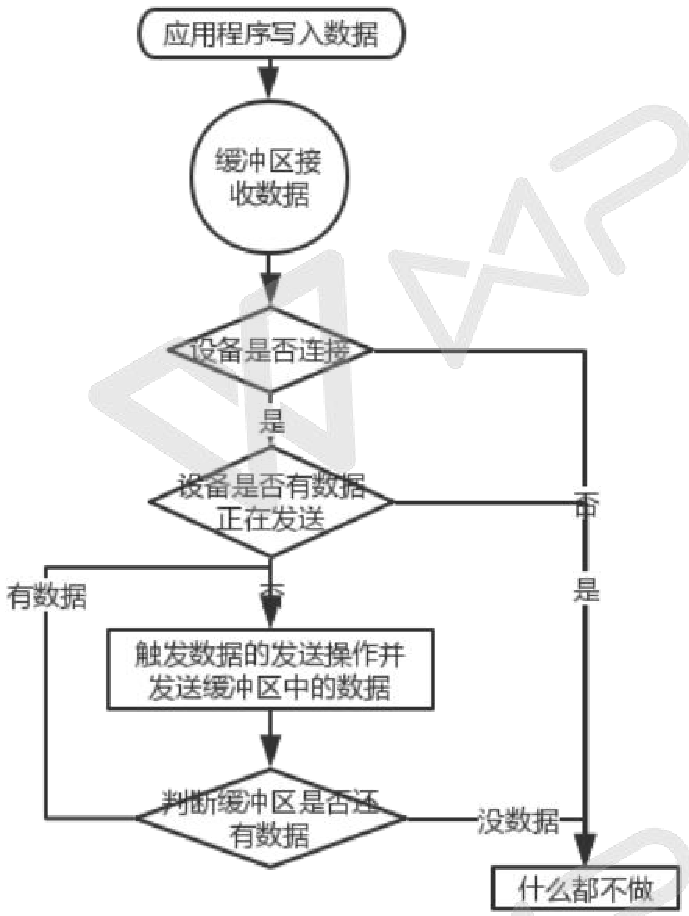
\includegraphics[width=.4\textwidth]{./graphics/outData-diagram.pdf}
\caption{数据发送逻辑图}\label{fig:outData-diagram}
\end{figure}

cp210xDevRead 和 cp210xDevWrite 的实现非常相似,只是更换了一下数据的传输方向。cp210xDevRead在底层也有一个循环缓冲区用来接收从USB口转串口设备发送来的数据,当需要读取 nbytes 个字节而缓冲区内的字节不够时,read就会阻塞,直到USBD层通知你有新的数据到来时才会继续进行读操作。同时也在驱动中启动了一个计时器,如果在计时器时间到了之后,还未能满足需要读取的字节数,则退出本次读写操作,返回当前已处理的字节数。


\subsubsection{设备的控制操作}
	设备控制简单的说用户对于设备某些工作行为的再配置。基于设备的类型,这些由驱动和 IO 子系统提供给用户的再配置参数会有所差别。Vxworks(其他通用操作系统也是如此)对各种类型的设备都抽取了一组共同属性作为配置选项,如串口波特率再配置就是一个串口标准属性。事实上,虽然有所约定,底层驱动完成可以虽然有所约定,底层驱动完成可以按照自己的标准对这些再配置属性进行选择:可以选择只实现其中某些再配置参数,可以按照特定设备的特殊情况选择对某个再配
置选项的响应方式或者转移再配置参数等等。可以说,设备控制函数既提供给了用户控制设备的方便性,也对底层设备的实现提供了极大的方便性,当然,底层驱动程序员不可以“欺骗”用户,必须完成用户要求的基本配置要求方可根据需要在做一些辅助性的配置工作,这是底层驱动设备控制实现函数的基本原则。

	除了 Vxworks 操作系统本身提供的控制参数外,对于一个特定设备也有自己的特定参数,这些也可以作为选项提供给用户进行控制。一般而言,底层驱动需要定义一个头文件,将设备特定参数在其中进行定义,而后将这个头文件提供给用户程序,当用户对设备进行操作时,其包含这个头文件,使用其中定义的特定参数对设备进行控制。IO 子系统实际上不加任何
改变的将用户使用的选项参数或者控制命令传递给了底层驱动,由底层驱动完成对选项参数或控制命令的解释和使用。
设备控制函数原型如下:
\lstset{language=C}
\begin{lstlisting}
LOCAL int cp210xDevIoctl(CP210X_DEV *pCp210xDev, int request, void *someArg )
\end{lstlisting}

对于我们的 USB口转串口S驱动,在实际使用中,再配置参数和命令有很多,但是目前我们只提供设备的波特率、数据位、校验位、流控的参数和命令。


\subsubsection{驱动卸载}
	在驱动的初始化中我们使用 iosDrvInstall 函数向 IO 子系统注册了我们的驱动,同时 IO 子系统也提供了另外一个相反作用的函数注销我们的驱动,这个函数就是 iosDrvRemove。该函数调用原型如下 :
\lstset{language=C}
\begin{lstlisting}
STATUS iosDrvRemove 
 ( 
 int drvnum, /* driver to remove, returned by iosDrvInstall()*/ 
 BOOL forceClose /* if TRUE, force closure of open files */ 
); 
\end{lstlisting}

该函数的第二个参数指定是否强制进行卸载,并将所有与此驱动有关的文件描述符关闭。如果强制关闭,则 IO 子系统将遍历系统文件描述符表,检查每个描述符对应结构中的驱动号是否等于要卸载驱动的驱动号,如果相同,则调用这个驱动的 close 实现函数进行关闭,同时释放文件描述符表中该表项,此时用户层的文件句柄将自动失去功效,如果用户其后使用这个文件描述符,将直接得到一个错误返回。

除了驱动卸载函数之外,我们的驱动初始化时还向USBD层进行了注册,在卸载的时候也应该注销USBD层的注册,同时注销动态注册的回调函数并从系统的设备表当中删除掉该设备。之后还应该对该驱动占用的所有其他的系统资源进行释放。



至此,我们已经完成了该特定需求下的USB口转串口驱动程序的所有组成部分的设计和实现。

\subsection{通用多设备驱动的实现}
